\documentclass[tikz,border=5mm]{standalone}
\usepackage{pgfplots}
\pgfplotsset{compat=1.16}

\begin{document}
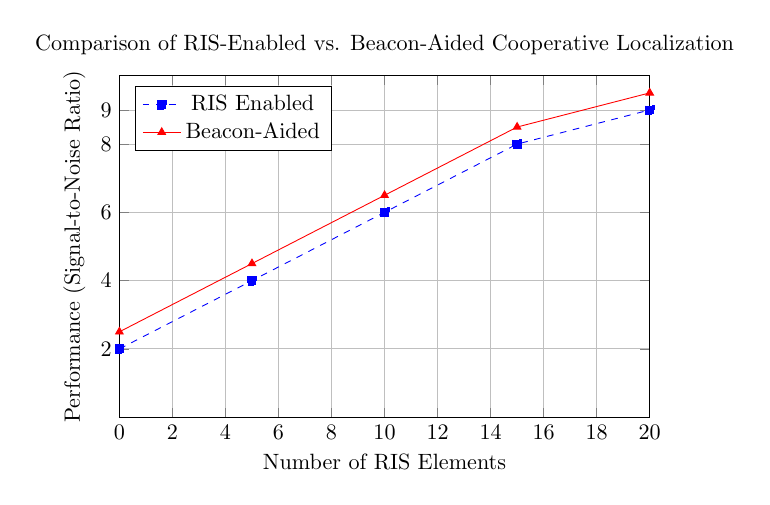
\begin{tikzpicture}[scale=0.8]
    \begin{axis}[
        xlabel={Number of RIS Elements},
        ylabel={Performance (Signal-to-Noise Ratio)},
        title={Comparison of RIS-Enabled vs. Beacon-Aided Cooperative Localization},
        xmin=0,
        xmax=20,
        ymin=0,
        ymax=10,
        ytick=data,
        grid=major,
        legend pos=north west,
        width=10cm,
        height=7cm
    ]
        % RIS Enabled Data
        \addplot[blue, mark=square*, dashed] coordinates {
            (0, 2)
            (5, 4)
            (10, 6)
            (15, 8)
            (20, 9)
        };
        \addlegendentry{RIS Enabled};

        % Beacon-Aided Data
        \addplot[red, mark=triangle*, solid] coordinates {
            (0, 2.5)
            (5, 4.5)
            (10, 6.5)
            (15, 8.5)
            (20, 9.5)
        };
        \addlegendentry{Beacon-Aided};
    \end{axis}
\end{tikzpicture}
\end{document}